% Requires running Bibtex

\documentclass[%
reprint,
amsmath,amssymb,
aps,
]{revtex4-2}

\usepackage{graphicx}% Include figure files
\usepackage{dcolumn}% Align table columns on decimal point
\usepackage{bm}% bold math
\usepackage{hyperref}% add hypertext capabilities
\usepackage[font=scriptsize,labelfont=bf, justification=justified]{caption}% change fontsize in captions
\usepackage{booktabs}% cool table style
\hypersetup{
	colorlinks=true,       % false: boxed links; true: colored links
	linkcolor=black,        % color of internal links
	citecolor=black,        % color of links to bibliography
	filecolor=black,     % color of file links
	urlcolor=black         
}

\usepackage{bibspacing}
\setlength{\bibitemsep}{.5\baselineskip plus .05\baselineskip minus .05\baselineskip}


\begin{document}
	
	\preprint{APS/123-QED}
	
	\title{PHYC30170 Physics with Astronomy and Space Science Lab 1;\\An Investigation of Surface Plasmon Resonance}
	
	\author{Daragh Hollman}
	\email{daragh.hollman@ucdconnect.ie}
	
	\date{\today}
	
	\begin{abstract}
		The aims of this experiment were to determine the excitation angle of the surface plasmon within the Kretschmann configuration and to investigate the dependence of surface plasmon resonance (SPR) on the wavelength of the incident light and the thickness of the silver foil. [NOT FINISHED]
	\end{abstract}

	\maketitle
	
	\section{Introduction}		
		Surface plasmons are transverse magnetic waves, comprised of oscillating electrons, which travel along the boundary of a metal and a dielectric \cite{undergradToledo}. They were first discovered in 1957 by R. H. Ritchie The study of surface plasmons is very important and has many applications in biophysics, particularly in the analysis of biomolecular interactions \cite{biomedicalApplications}, and in many fields of optics including but not limited to sub-wavelength optics and near-field optics \cite{opticalApplications}.
	
	\section{Theory}
		\subsection{Excitation of Free Electrons}
			\url{https://iopscience-iop-org.ucd.idm.oclc.org/article/10.1088/0022-3727/45/11/113001}
		
		\subsection{Surface Plasmon Waves}
		
		\subsection{Apparatus}
			The apparatus was set up as shown in figure \ref{fig:apparatus}. More specifically, the Kretschmann configuration was used, figure \ref{fig:kConfig}.
			
			
			External vs internal angle
			\begin{figure}
				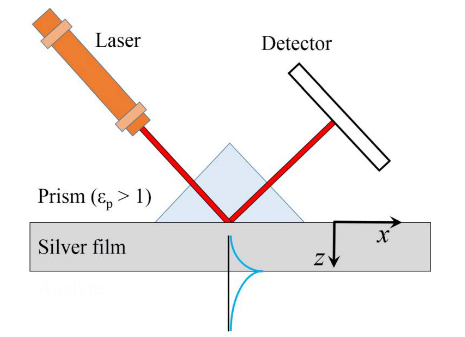
\includegraphics[width=0.9\columnwidth]{kConfig.png}
				\caption{\label{fig:kConfig} The Kretschmann configuration. The silver film was evaporated onto the glass prism. The light from the laser excites the plasmons on the outer side of the film. \cite{opticalApplications}}
			\end{figure}
		
			\begin{figure}
				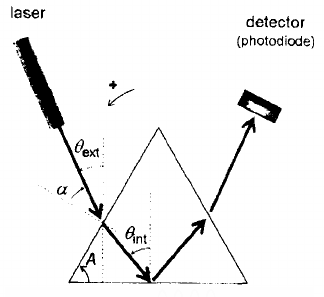
\includegraphics[width=0.9\columnwidth]{anglesDiagram.png}
				\caption{\label{fig:angles} A diagram describing the external and internal angles \cite{pluchery}.}
			\end{figure}
	 
	\section{Methodology}
		\subsection{Apparatus Setup}
			The apparatus was set up in the Kretschmann configuration as shown in figure \ref{fig:kConfig}. A silver film was evaporated onto three prisms so that the thickness of the film could be varied. Thicknesses of 10nm, 13nm, and 15nm were used. The prism was placed in the centre of a bidirectional stepping rotary table. This table had two independently movable discs (specifically one disc and one annulus) controlled by stepper motors which, through a gear system, had a precision calibrated to be $0.045$ degrees per step. The prism was placed on the inner disc and a photodiode was fixed on the outer annulus to be used as a detector.\\
			
			The apparatus was controlled using Python 3 to interface with a USB multifunction I/O device, NI USB-6009 \cite{nationalInstruments}. This was used as a digital to analogue converter to control the stepper motors as well as an input from the photodiode to read voltages. A laser was placed into a retort stand such that it would pass through the prism and reflect off the silver film into the photodiode.

			\subsubsection{Light Source}
				Three He-Ne lasers were used of wavelengths 633nm, 515nm, and 405nm all of which had a maximum power $\le 4 \,\text{mW}$. In this report we will refer to these lasers as red, green, and blue respectively. A linear polarising filter was positioned between the laser and the prism such to p-polarise the incident light.
			
			\subsubsection{Motor Programming}
				The stepper motor modules were programmed following the documentation provided by UCD \cite{motorDoc}. They were controlled by digital signals to the control lines of the USB I/O device. The control lines were used to enable and disable the motors, set the direction, and to advance each motor. We initially had issues getting these inputs to work as one of the pins was wired incorrectly, however through exhaustive testing we were able to identify the correct pins for each input. A function was then written in Python to control the movement of these motors. This function took inputs of a number of steps, a direction, and a delay time. It was important to include a short delay ($\approx 100\,\text{ms}$) between steps to reduce unwanted vibrational artefacts in the data and to not overheat the motors. Functionality was also included to select to rotate either the prism, or the detector, or both. This function is included in appendix A.1 on data acquisition.
			
			\subsubsection{Developing an Algorithm for Data Collection}
				This function was then edited to include capabilities to include data collection from the photodiode while moving. After each step 100 samples of the voltage were taken at $10,000\,\text{Hz}$. The mean of these was recorded as the voltage value and the standard deviation was taken as the uncertainty.\\
				
				To improve efficiency, functionality to drive the system backwards as well as forwards was introduced to remove the time taken to reset the apparatus to its initial position.\\
				
				Note that the detector had to move twice for every prism step to keep the laser tracked on the detector. This was due to their separation.

			\subsubsection{Laser Alignment}
				The laser, detector, and prism were aligned such that the right angled side of the prism was facing towards the laser and the beam was reflected back towards itself. We define this as an external angle of $0$ degrees. This was then moved $20$ degrees clockwise and the detector was moved into the path of the reflected beam.
			
		\subsection{Data Collection}
			\subsubsection{}
		
		
	
	\section{Results and Analysis}
		\subsection{Varying Laser Wavelength}
		
		\subsection{Varying Metal Thickness}
	
		\subsection{Anomaly found during Red Laser Runs}

	\section{Conclusion}
		
		
	\newpage
	\bibliography{surfacePlasmons}% Produces the bibliography via BibTeX.
		
	\newpage
	\appendix
		
	\section{Python Code}
	
		\subsection{Data Acquisition}
		
		\subsection{Analysis}
		
\end{document}

